\section{Theories Beyond the Standard Model}\label{sec:bsm}
Theories beyond the Standard Model (BSM) can be used to explain anomalous observations such as dark matter~\cite{Clowe:2006eq}, and to solve theoretical problems like the hierarchy problem~\cite{Thomson:2013zua}. In this section, three theories (or families of theories) relevant to the experimental work presented in this thesis are discussed: Warped Extra Dimensions (WED), the Next-to-Minimal-Supersymmetric Standard Model (NMSSM), and Effective Field Theories (EFTs).

\subsection{Warped Extra Dimensions}\label{sec:wed}
In the Warped Extra Dimensions (WED) model~\cite{Randall:1999ee,Carvalho:2014lsg}, a five-dimensional geometry is proposed where a small spatial dimension is added to the traditional 4D spacetime. This theory alleviates the hierarchy problem and introduces two new \textit{gravity particles}: a spin-0 boson called the Radion which we denote \XZero, and a spin-2 boson called the Graviton which we denote \XTwo. Two theoretical scenarios are described in Ref.~\cite{Carvalho:2014lsg}, one where the SM particles are not allowed to propagate along the extra dimension and another where they are allowed, and these scenarios are referred to as the RS1 and Bulk scenarios respectively.

The decay channels and branching fractions for the Radion and Graviton are shown in \cref{fig:WED_BF}. In the Bulk scenario, the branching fraction to two SM Higgs bosons is about 30\% and about 10\% for the Radion and Graviton respectively for masses above 300\GeV. There are higher branching fractions to other decay channels such as \WW but more sensitive searches can be achieved with \HH if the right Higgs boson decay channels are chosen. One of the most competitive \HH decay channels is $b\bar{b}\gamma\gamma$ which has lower backgrounds and better mass resolution compared to $\PX \to \PW\PW$. 

Even better constraints can be achieved by performing searches with additional Higgs boson decay channels and then combining these searches, and this motivates the \XHH search in the $\gamma\gamma\tau\tau$ final state presented in \cref{chap:dihiggs}. In the RS1 scenario, the $\XTwo \to \PH\PH$ decay channel has a significantly lower branching fraction of around $\sim0.5\%$. Therefore, the search in \cref{chap:dihiggs} only considers the Bulk scenario. Production cross sections for the Radion and Graviton at $\sqrt{s}=13\TeV$ in the Bulk scenario are shown in \cref{fig:WED_xs} for particular values of $kl$, $\Lambda_R$ and $\tilde{k}$ which are free parameters of the theory and described in Ref.~\cite{Carvalho:2014lsg}. The dominant production mode for both the Radion and Graviton is gluon-gluon fusion.

\begin{figure}
  \centering
  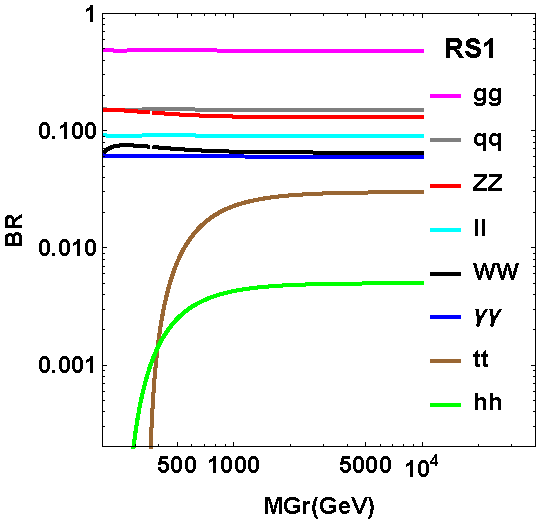
\includegraphics[width=0.49\textwidth]{Figures/Theory/WED/RSGravitonBRanal.pdf}
  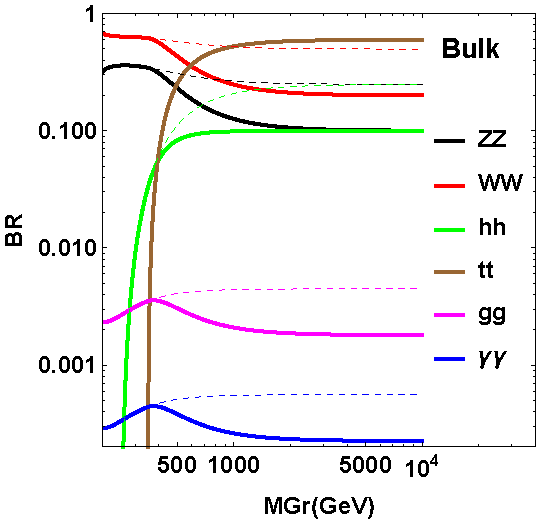
\includegraphics[width=0.49\textwidth]{Figures/Theory/WED/BulkGravitonBRanalWitTop.pdf}
  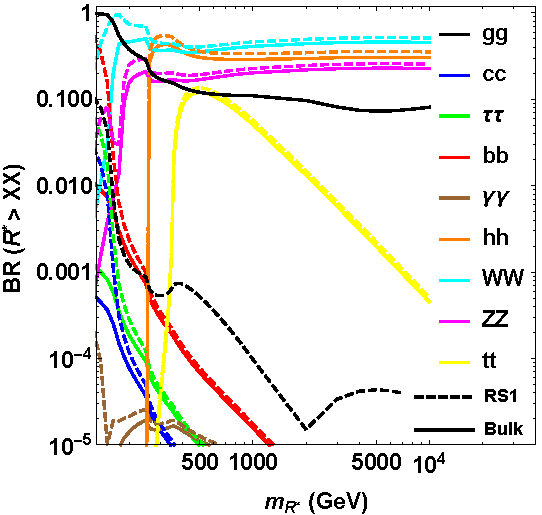
\includegraphics[width=0.49\textwidth]{Figures/Theory/WED/BR_eHDecay.pdf}
  \caption[Graviton and Radion Branching Fractions]{Branching fractions for the Graviton (top) and Radion (bottom) as functions of the particle masses. The RS1 and Bulk scenarios for the Graviton are shown in the top-left and top-right respectively whereas for the Radion, they are shown on the same plot and are differentiated by dashed and solid lines respectively. Figures are taken from Ref.~\cite{Carvalho:2014lsg}.}\label{fig:WED_BF}
\end{figure}

\begin{figure}
  \centering
  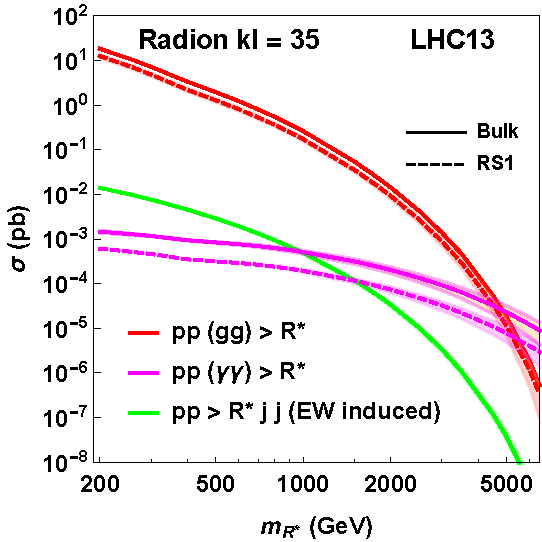
\includegraphics[width=0.48\textwidth]{Figures/Theory/WED/CX_RS_radion_13tev.pdf}
  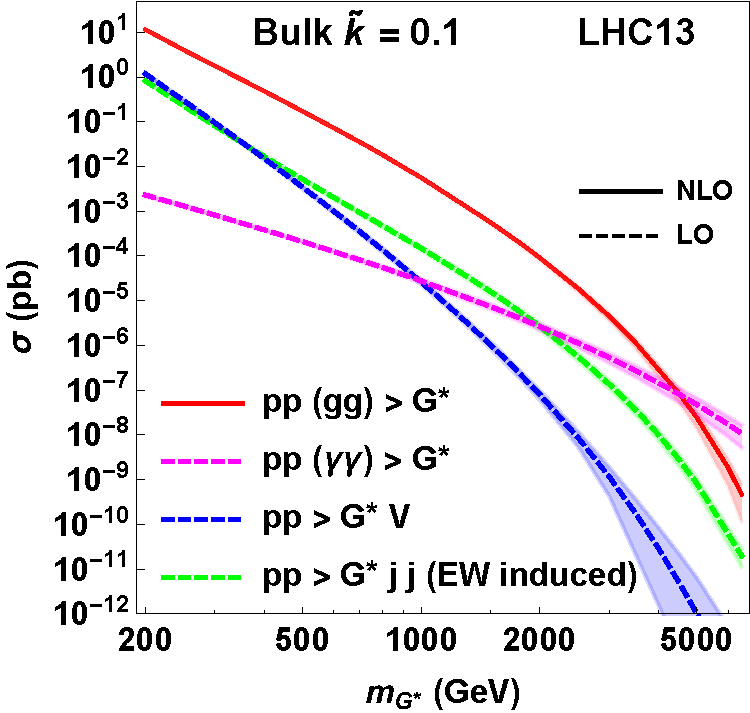
\includegraphics[width=0.49\textwidth]{Figures/Theory/WED/CX_bulk_13tev.pdf}
  \caption[Graviton and Radion Production Cross Sections]{Production cross sections at the LHC with $\sqrt{s}=13\TeV$ for the Radion ($R^*$) on the left, and the Graviton ($G^*$) on the right, shown as functions of the resonance masses. The Radion cross sections are shown for $kl=35$ and $\Lambda_R=3$\TeV and the Graviton cross sections are shown for $\tilde{k}=0.1$. Figures are taken from Ref.~\cite{Carvalho:2014lsg}.}\label{fig:WED_xs}
\end{figure}


\subsection{The Next-to-Minimal-Supersymmetric Standard Model}\label{sec:susy}
In supersymmetric theories, every SM particle has a \textit{superpartner} which differs in spin by $1/2$. In other words, every SM boson has a fermionic superpartner, and every SM fermion has a bosonic superpartner. Supersymmetric extensions of the SM are motivated by a solution to the hierarchy problem, an automatic unification of the running gauge couplings at a Grand Unified (GUT) scale $M_{\text{GUT}}$, and the introduction of a stable neutral particle which can be identified as a dark matter candidate~\cite{Ellwanger:2009dp}. 

In the Minimal Supersymmetric Standard Model (MSSM), there are two Higgs \SU{2}-doublets, $\Phi_1$ and $\Phi_2$, which lead to three neutral and two charged Higgs bosons~\cite{Fayet:1974pd,Fayet:1977yc}. An unattractive property of the MSSM is that the Lagrangian must contain a supersymmetric mass term for the Higgs doublets, which has to be of the order of the SUSY breaking scale, $M_{\text{SUSY}}$, for phenomenological reasons. Ideally, the electroweak scale generated by the Higgs vevs would depend only on $M_{\text{SUSY}}$, which would be the only remaining scale asking for an explanation as to why it is far below $M_{\text{GUT}}$ or the Planck scale $M_{\text{Planck}}$. This issue with the MSSM, denoted as the ``$\mu$-problem'', is rectified in the Next-to-Minimal Supersymmetric Standard Model (NMSSM)~\cite{Ellwanger:2009dp} and the solution requires the introduction of a singlet field, $S$. Models with this scalar structure are referred to as two-Higgs-doublet + singlet models (2HDM+S).

In 2DMH+S models, there are 3 CP-even and 2 CP-odd neutral scalars, and in the gauge eigenbasis these are denoted $H^{\text{SM}}$, $H^{\text{NSM}}$, $H^{\text{S}}$ and $A^{\text{NSM}}$, $A^{\text{S}}$ for the CP-even and CP-odd bosons respectively. The couplings of these states to SM particles are:
\begin{align*}
    H^{\text{SM}}(f_1,f_2,\mathrm{VV}) &= (g_{\text{SM}}, g_{\text{SM}}, g_{\text{SM}}), \\
    H^{\text{NSM}}(f_1,f_2,\mathrm{VV}) &= (g_{\text{SM}}/\tan{\beta}, -g_{\text{SM}}\tan{\beta}, 0), \\
    H^{\text{S}}(f_1,f_2,\mathrm{VV}) &= (0,0,0), \\
    A^{\text{NSM}}(f_1,f_2,\mathrm{VV}) &= (g_{\text{SM}}/\tan{\beta}, -g_{\text{SM}}\tan{\beta}, 0), \\
    A^{\text{S}}(f_1,f_2,\mathrm{VV}) &= (0,0,0)
\end{align*}
where $f_1$ ($f_2$) are SM fermions that couple to $\Phi_1$ ($\Phi_2$), $\mathrm{VV}$ corresponds to pairs of $\mathrm{W}$ or $\mathrm{Z}$ bosons, $g_{\text{SM}}$ is the coupling of a SM Higgs boson to such particles, and $\tan{\beta}$ is the ratio of vacuum expectation values: $\tan{\beta}=v_1/v_2$ where $v_1\equiv \langle \Phi_1 \rangle$ and  $v_2 \equiv \langle \Phi_2 \rangle$~\cite{Baum:2018zhf}.

The CP-even and CP-odd mass eigenstates obtained after mixing of gauge eigenstates are denoted $h_i=\{h_{125},H,h\}$ and $a_i=\{A,a\}$ respectively where $h_{125}$ is identified as the 125 GeV SM-like state observed at the LHC. The mass ordering is such that $m_H>m_h$ and $m_A>m_a$. In the alignment limit where $h_{125} = H^{\text{SM}}$, couplings for interactions involving $h_{125}h_{125}$ and one of the other scalars go to zero. On the other hand, couplings for $Hhh_{125}$ and $Aah_{125}$ are non-zero, which allows for so-called \textit{cascade decays}: $H\rightarrow h h_{125}$ and $A \rightarrow a h_{125}$. This motivates the \XYH search in \cref{chap:dihiggs} where \PX and \PY are new scalars, and \PH is the SM Higgs boson.

\subsubsection{$Y\rightarrow \gamma\gamma$ in the NMSSM at Low \mY}\label{sec:low_mass_in_NMSSM}

\begin{figure}
    \centering
    \inputtikz{Figures/Theory/SUSY/a_gamgam.tex}
    \caption[Feynman Diagram for a CP-Odd Higgs Boson Decaying to Two Photons Via a Chargino Loop]{Feynman diagram for the decay of the CP-odd Higgs boson, $a$, to two photons mediated by a chargino ($\chi^\pm$) loop.}\label{fig:a_gamgam}
   \end{figure}

If the lightest CP-odd Higgs in the mass basis, $a$, is very singlet-like, i.e.\ its main component is $A^S$, then its couplings to SM particles are heavily suppressed, and therefore, the typical hierarchy of Higgs decays: $bb, WW, \tau\tau, ZZ,\ldots$ becomes irrelevant. It is still possible for $a$ to decay to SM particles through loop interactions (see \cref{fig:a_gamgam}). The Higgs decay to two photons, which is suppressed in the SM, can now become the dominant decay mode for $a$, with a branching fraction up to 85\% depending on the theoretical scenario~\cite{King:2014xwa}. Since $a$ couples weakly to SM particles, its direct production, $pp \to a$ is also suppressed. The couplings of $a$ to BSM particles are however, not suppressed. Therefore, a search for $pp \rightarrow A \rightarrow a h_{125}$, where $a\to\gamma\gamma$, is uniquely placed to study this region of the NMSSM phase space. This motivates the inclusion of \Ygg in the \XYH search in \cref{chap:dihiggs}. 

In Ref.~\cite{Ellwanger:2022jtd}, maximally-allowed cross sections for this process are calculated given constraints from a set of relevant measurements. These cross sections are shown in \cref{fig:max_allowed_constraints}. If in the search for this process, we can set upper limits for the cross sections below the maximally-allowed, it means that our search will provide tighter constraints on the NMSSM than available at the time that Ref.~\cite{Ellwanger:2022jtd} was published (May 2022).

\begin{figure}[h]
    \centering
    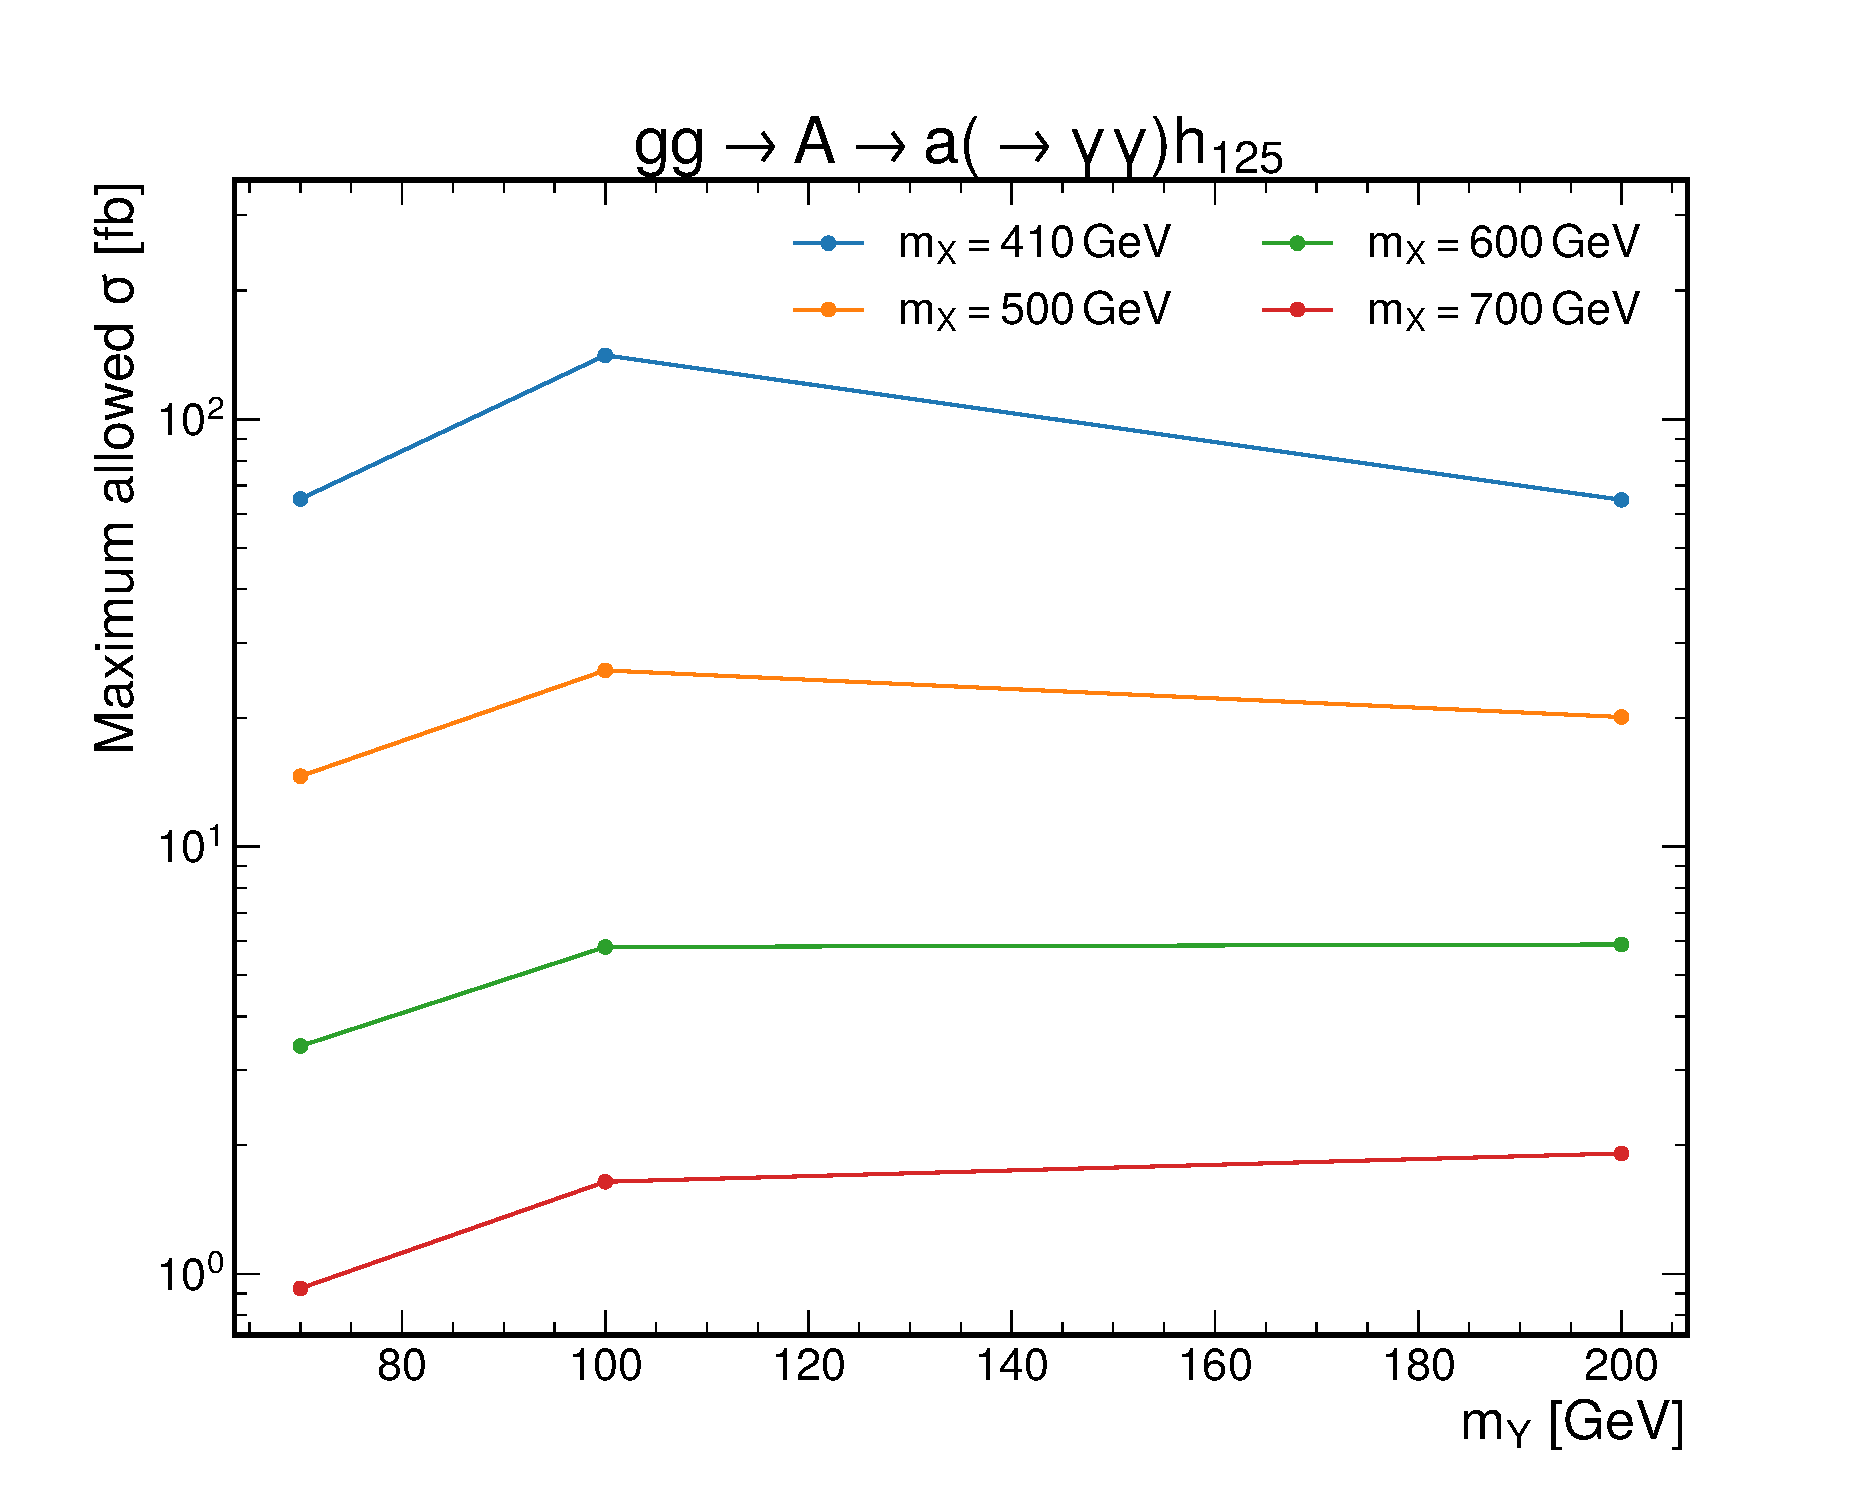
\includegraphics[width=0.7\textwidth]{Figures/Theory/SUSY/max_allowed_limits.pdf}
    \caption[Maximally-Allowed Cross Sections for $pp\rightarrow A \rightarrow H_{125}(\rightarrow\tau\tau)a(\rightarrow\gamma\gamma)$ in the NMSSM]{Maximally-allowed cross sections for $pp\rightarrow A \rightarrow h_{125}a(\rightarrow\gamma\gamma)$ in the NMSSM provided experimental constraints~\cite{Ellwanger:2022jtd}.}\label{fig:max_allowed_constraints}
\end{figure}
\newpage
\subsection{Effective Field Theory}\label{sec:EFT}
\subsubsection{Fermi Theory}

An effective field theory (EFT) is a low-energy approximation of another theory that is capable of making accurate predictions up to a particular energy scale. For example, the weak interaction can be approximated by an EFT called Fermi theory~\cite{Fermi:1934hr} which contains no description of the \PW or \PZ bosons. In the SM, muon decay is mediated by the exchange of a \PW boson but in Fermi theory, this is calculated using a four-point interaction (see \cref{fig:muon_decay_diagrams}). 

\begin{figure}
  \centering
  \inputtikz{Figures/Theory/EFT/muon_decay_sm.tex}
  \hspace{1cm}
  \inputtikz{Figures/Theory/EFT/muon_decay_fermi.tex}
  \caption[LO Feynman Diagrams for Muon Decay in the SM and in Fermi Theory]{LO Feynman diagrams for muon decay in the SM (left) and in Fermi theory (right).}\label{fig:muon_decay_diagrams}
\end{figure}

In the SM diagram, the mediating \PW boson, which is also referred to as a \textit{propagator}, introduces a term to the matrix element:
\begin{equation}
  \mathcal{M} = - i \frac{g_\mn - \frac{q_\mu q_\nu}{m_\PW^2}}{q^2 - m_\PW^2 + im_\PW \Gamma_\PW} \times \cdots
\end{equation}
where $q$ is the four-vector of the momentum transferred by the \PW boson, $\Gamma_\PW=2.09\GeV$ is the decay width of the \PW boson, and $g_\mn$ is the Minkowski metric.
In muon decay, $\sqrt{q^2} \ll m_\PW$ since $q^2 = m_\mu^2$ and given that $\Gamma_\PW \ll m_\PW$ as well, the propagator term is approximately:
\begin{equation}
  \frac{i g_\mn}{m_\PW^2}
\end{equation}
which, ignoring the vector indices, is a constant and can be absorbed into the coupling strength parameter of the Fermi theory, i.e.\ the theories are the same except for a factor of $1/m_\PW^2$ in the coupling strengths. The full calculation in Fermi theory predicts the decay width to be:
\begin{equation}
  \Gamma = \frac{G_F^2}{(\hbar c)^6}\frac{(m_\mu c^2)^5}{192 \pi^3}
\end{equation}
where $G_F$ is the \textit{Fermi constant} which characterizes the strength of the interaction. This can be related to the electroweak \SU{2} coupling, $g_2$, with:
\begin{equation}
  G_F = \frac{1}{4\sqrt{2}} \frac{g_2^2}{m_\PW^2}
\end{equation}
and therefore, a measurement of the muon decay width provides a relationship between the couplings of the weak interaction and the \PW boson mass. 

More generally, an interaction involving a propagator can be approximated by a point interaction if $q^2 \ll \Lambda^2$ where $\Lambda$ is the mass of the propagator. Then, measurements of interactions in that energy regime can be used to place constraints on the relationship between $g$ and $\Lambda$, where $g$ is a coupling parameter for these interactions. This extends to propagators outside the SM and therefore, EFT can be used to place constraints on new physics when using measurements at an energy scale much less than the mass of the new particle. 

\subsubsection{Standard Model Effective Field Theory}

The Standard Model Effective Field Theory (SMEFT) extends the SM Lagrangian by adding terms of higher dimension:
\begin{equation}
  \LSMEFT = \LSM + \frac{1}{\Lambda} \sum_i C_i^{(5)} O_i^{(5)} + \frac{1}{\Lambda^2} \sum_i C_i^{(6)} O_i^{(6)} + \cdots
  \label{eq:LSMEFT}
\end{equation}
where $O_i^{(d)}$ are dimension-$d$ terms called \textit{operators} that contain the SM fields and are invariant under the same gauge group as the SM, and $C_i^{(d)}$ are complex numbers called \textit{Wilson coefficients} that characterize the magnitude of each operator's contribution to \LSMEFT. Since \LSMEFT is a perturbative expansion, it requires that $C_i / \Lambda^d < \mathcal{O}(1)$ for all $C_i$.

We neglect all operators that violate lepton-number or baryon-number conservation and any operators that are dimension-7 or higher since they are suppressed by higher orders of $1 / \Lambda$. At dimension five, one operator remains which generates a Majorana mass term for neutrinos, and we also neglect this. The rest of this section will focus on the remaining dimension-6 terms which we denote by \Lsix.

We use a non-redundant basis for the operators called the Warsaw basis~\cite{Grzadkowski:2010es}. The basis definition is written in \cref{tab:Warsaw_basis}, using the following notation:
\begin{align}
  \tilde{X}^\mn &= \frac{1}{2} \epsilon^{\mn\rho\sigma} X_{\rho\sigma}, \quad &&H^\dag i \overleftrightarrow{D} H = H^\dag (i D_\mu H) - (i D_\mu H^\dag) H, \\
  \sigma^\mn &= \frac{i}{2} [\gamma^\mu, \gamma^\nu], &&H^\dag i \overleftrightarrow{D}^i H = H^\dag \sigma^i (i D_\mu H) - (i D_\mu H^\dag) \sigma^i H .
\end{align}

\clearpage
\thispagestyle{empty}
\begin{table}[h!]
  \begin{center}
  \small
  \hspace*{-2cm}
   \renewcommand{\arraystretch}{1.7}
   \begin{tabular}{|*3{>{$}c<{$}|>{$}p{4cm}<{$}|}}
  
   \toprule
   \multicolumn{2}{|c|}{$\mathcal{L}_6^{(1)}$ -- $X^3$} & 
    \multicolumn{2}{c|}{$\mathcal{L}_6^{(6)}$ -- $\psi^2 XH$}&
   \multicolumn{2}{c|}{$\mathcal{L}_6^{(8b)}$ -- $(\bar RR)(\bar RR)$}
   \\
  \midrule
  % c1
  Q_G & 
  f^{abc} G_\mu^{a\nu} G_\nu^{b\rho} G_\rho^{c\mu}  &
  % c6 
  Q_{eW} & 
  (\bar l_p \sigma^{\mu\nu} e_r) \sigma^i H W_{\mu\nu}^i &
  % 8b
  Q_{ee} & 
  (\bar e_p \gamma_\mu e_r)(\bar e_s \gamma^\mu e_t) 
  \\
  % c1
  Q_{\widetilde G} & 
  f^{abc} \widetilde G_\mu^{a\nu} G_\nu^{b\rho} G_\rho^{c\mu}  &
  % c6 
  Q_{eB} & 
  (\bar l_p \sigma^{\mu\nu} e_r) H B_{\mu\nu} &
  % 8b
  Q_{uu} & 
  (\bar u_p \gamma_\mu u_r)(\bar u_s \gamma^\mu u_t) 
  \\
  % c1
  Q_W & 
  \epsilon^{ijk} W_\mu^{i\nu} W_\nu^{j\rho} W_\rho^{k\mu} &
  % c6 
  Q_{uG} & 
  (\bar q_p \sigma^{\mu\nu} T^a u_r) \widetilde H \, G_{\mu\nu}^a &
  % 8b
  Q_{dd} & 
  (\bar d_p \gamma_\mu d_r)(\bar d_s \gamma^\mu d_t) 
  \\
  % c1
  Q_{\widetilde W}& 
  \epsilon^{ijk} \widetilde W_\mu^{i\nu} W_\nu^{j\rho} W_\rho^{k\mu} &
  % c6 
  Q_{uW} & 
  (\bar q_p \sigma^{\mu\nu} u_r) \sigma^i \widetilde H \, W_{\mu\nu}^i &
  % 8b
  Q_{eu} & 
  (\bar e_p \gamma_\mu e_r)(\bar u_s \gamma^\mu u_t) 
  \\\cline{1-2}
   \multicolumn{2}{|c|}{$\mathcal{L}_6^{(2)}$ -- $H^6$} &
  % c6 
  Q_{uB} & 
  (\bar q_p \sigma^{\mu\nu} u_r) \widetilde H \, B_{\mu\nu} &
  % 8b
  Q_{ed} & 
  (\bar e_p \gamma_\mu e_r)(\bar d_s\gamma^\mu d_t) 
  \\\cline{1-2}
  % c2
  Q_H & 
  (H^\dag H)^3 &
  % c6 
  Q_{dG} & 
  (\bar q_p \sigma^{\mu\nu} T^a d_r) H\, G_{\mu\nu}^a &
  % 8b
  Q_{ud}^{(1)} & 
  (\bar u_p \gamma_\mu u_r)(\bar d_s \gamma^\mu d_t) 
  \\
  \cline{1-2}
  \multicolumn{2}{|c|}{$\mathcal{L}_6^{(3)}$ -- $H^4 D^2$} &
  % c6 
  Q_{dW} & 
  (\bar q_p \sigma^{\mu\nu} d_r) \sigma^i H\, W_{\mu\nu}^i &
  % 8b
  Q_{ud}^{(8)} & 
  (\bar u_p \gamma_\mu T^a u_r)(\bar d_s \gamma^\mu T^a d_t) 
  \\\cline{1-2}
  % c3
  Q_{H\Box} & 
  (H^\dag H)\Box(H^\dag H) &
  % c6 
  Q_{dB} & 
  (\bar q_p \sigma^{\mu\nu} d_r) H\, B_{\mu\nu} &
  % c8b
  &
  \\
  % c3
  Q_{H D} & 
  \ \left(D^\mu H^\dag  H\right) \left(H^\dag D_\mu H\right) &
  %c6
  &&
  % c8b
  &
  \\\midrule
   \multicolumn{2}{|c|}{$\mathcal{L}_6^{(4)}$ -- $X^2H^2$}& 
   \multicolumn{2}{c|}{$\mathcal{L}_6^{(7)}$ -- $\psi^2H^2 D$}& 
   \multicolumn{2}{c|}{$\mathcal{L}_6^{(8c)}$ -- $(\bar LL)(\bar RR)$}
  \\\midrule
  % c4
  Q_{H G}  & 
  H^\dag H\, G^a_{\mu\nu} G^{a\mu\nu} &
  % c7
  Q_{H l}^{(1)} & 
  (H^\dag i\overleftrightarrow{D}_\mu H)(\bar l_p \gamma^\mu l_r)&
  % 8c
  Q_{le} & 
  (\bar l_p \gamma_\mu l_r)(\bar e_s \gamma^\mu e_t)
  \\
  % c4
  Q_{H\widetilde G} & 
  H^\dag H\, \widetilde G^a_{\mu\nu} G^{a\mu\nu} &
  % c7
  Q_{H l}^{(3)} & 
  (H^\dag i\overleftrightarrow{D}^i_\mu H)(\bar l_p \sigma^i \gamma^\mu l_r)&
  % 8c
  Q_{lu} & 
  (\bar l_p \gamma_\mu l_r)(\bar u_s \gamma^\mu u_t) 
  \\
  % c4
  Q_{H W} & 
  H^\dag H\, W^i_{\mu\nu} W^{I\mu\nu} &
  % c7
  Q_{H e} & 
  (H^\dag i\overleftrightarrow{D}_\mu H)(\bar e_p \gamma^\mu e_r)&
  % 8c
  Q_{ld} & 
  (\bar l_p \gamma_\mu l_r)(\bar d_s \gamma^\mu d_t) 
  \\
  % c4
  Q_{H\widetilde W} & 
  H^\dag H\, \widetilde W^i_{\mu\nu} W^{i\mu\nu} &
  % c7
  Q_{H q}^{(1)} & 
  (H^\dag i\overleftrightarrow{D}_\mu H)(\bar q_p \gamma^\mu q_r)&
  % 8c
  Q_{qe} & 
  (\bar q_p \gamma_\mu q_r)(\bar e_s \gamma^\mu e_t)
  \\
  % c4
  Q_{H B} &  H^\dag H\, B_{\mu\nu} B^{\mu\nu} &
  % c7
  Q_{H q}^{(3)} & 
  (H^\dag i\overleftrightarrow{D}^i_\mu H)(\bar q_p \sigma^i \gamma^\mu q_r)&
  % 8c
  Q_{qu}^{(1)} & 
  (\bar q_p \gamma_\mu q_r)(\bar u_s \gamma^\mu u_t)
  \\
  % c4
  Q_{H\widetilde B} & 
  H^\dag H\, \widetilde B_{\mu\nu} B^{\mu\nu} &
  % c7
  Q_{H u} & 
  (H^\dag i\overleftrightarrow{D}_\mu H)(\bar u_p \gamma^\mu u_r)&
  % 8c
  Q_{qu}^{(8)} & 
  (\bar q_p \gamma_\mu T^a q_r)(\bar u_s \gamma^\mu T^a u_t) 
  \\
  % c4
  Q_{H WB} & 
   H^\dag \sigma^i H\, W^i_{\mu\nu} B^{\mu\nu} &
  % c7
  Q_{H d} & 
  (H^\dag i\overleftrightarrow{D}_\mu H)(\bar d_p \gamma^\mu d_r)&
  % 8c
  Q_{qd}^{(1)} & 
  (\bar q_p \gamma_\mu q_r)(\bar d_s \gamma^\mu d_t) 
  \\
  % c4
  Q_{H\widetilde W B} & 
  H^\dag \sigma^i H\, \widetilde W^i_{\mu\nu} B^{\mu\nu} &
  % c7
  Q_{H u d}+\hc & 
  i(\widetilde H ^\dag D_\mu H)(\bar u_p \gamma^\mu d_r)&
  % 8c
  Q_{qd}^{(8)} & 
  (\bar q_p \gamma_\mu T^a q_r)(\bar d_s \gamma^\mu T^a d_t)
  \\
  \midrule
   \multicolumn{2}{|c|}{$\mathcal{L}_6^{(5)}$ -- $\psi^2 H^3$} &
   \multicolumn{2}{c|}{$\mathcal{L}_6^{(8a)}$ -- $(\bar LL)(\bar LL)$}&
   \multicolumn{2}{c|}{$\mathcal{L}_6^{(8d)}$ -- $(\bar LR)(\bar RL)$, $(\bar LR)(\bar LR)$} 
   \\\midrule
  % c5
  Q_{eH} & 
  (H^\dag H)(\bar l_p e_r H) &
  % 8a 
  Q_{ll}  & 
  (\bar l_p \gamma_\mu l_r)(\bar l_s \gamma^\mu l_t)&
  % 8d
  Q_{ledq} & 
  (\bar l_p^j e_r)(\bar d_s q_{tj})
  \\
  % c5
  Q_{uH}  &
  (H^\dag H)(\bar q_p u_r \widetilde H )&
  % 8a
  Q_{qq}^{(1)} & 
  (\bar q_p \gamma_\mu q_r)(\bar q_s \gamma^\mu q_t) &
  % 8d 
  Q_{quqd}^{(1)} & 
  (\bar q_p^j u_r) \epsilon_{jk} (\bar q_s^k d_t) 
  \\
  % c5
  Q_{dH}  & 
  (H^\dag H)(\bar q_p d_r H)&
  % 8a 
  Q_{qq}^{(3)} & 
  (\bar q_p \gamma_\mu \sigma^i q_r)(\bar q_s \gamma^\mu \sigma^i q_t) &
  % 8d
  Q_{quqd}^{(8)} & 
  (\bar q_p^j T^a u_r) \epsilon_{jk} (\bar q_s^k T^a d_t) 
  \\
  % c5
  &&
  % 8a 
  Q_{lq}^{(1)} & 
  (\bar l_p \gamma_\mu l_r)(\bar q_s \gamma^\mu q_t)&
  % 8d
  Q_{lequ}^{(1)} & 
  (\bar l_p^j e_r) \epsilon_{jk} (\bar q_s^k u_t) 
  \\
  % c5
  &&
  % 8a 
  Q_{lq}^{(3)} & 
  (\bar l_p \gamma_\mu \sigma^i l_r)(\bar q_s \gamma^\mu \sigma^i q_t) &
  % 8d
  Q_{lequ}^{(3)} & 
  (\bar l_p^j \sigma_{\mu\nu} e_r) \epsilon_{jk} (\bar q_s^k \sigma^{\mu\nu} u_t) 
  \\\bottomrule
  \end{tabular}
  % }
  \end{center}
  \caption[Warsaw Basis of Operators]{$\mathcal{L}_6$ operators in the Warsaw basis~\cite{Grzadkowski:2010es}, categorized into eight classes $\mathcal{L}_6^{(n)}$ as in~\cite{Alonso:2013hga}. Only baryon number-conserving invariants are retained. The flavor indices $p,r,s,t$ are suppressed in the operators' labels.}\label{tab:Warsaw_basis}
  \end{table}

In \cref{tab:Warsaw_basis}, there are 59 independent operators and naively, one might expect therefore, that there are only 59 Wilson coefficients that need to be measured to specify the theory. However, some operators carry flavour indices of which all combinations need to be summed over:
\begin{equation}
  \Lsix = \frac{1}{\Lambda^2} \sum_i \sum^3_{p,r=1} C_{i,pr} Q_{i,pr} + \cdots
  \label{eq:smeft_flavour_combinations}
\end{equation}
and this leads to a higher number of Wilson coefficients. In total, there are 2599 free parameters in \Lsix, counting real and imaginary components of the Wilson coefficients separately. It is not currently possible to experimentally constrain all of these parameters simultaneously and nor will it be in the short-term future. Therefore, we use flavour assumptions to reduce the number of free parameters to a more reasonable level.

\subsubsection{Flavour Assumptions}
The most restrictive flavour assumption we can make is the symmetry of the kinetic terms: $\U{3}^5 = \U{3}_q \times \U{3}_u \times \U{3}_d \times \U{3}_l \times\U{3}_e$, where each field is assigned to a three-component representation of the associated group. In this assumption, the terms in \cref{eq:smeft_flavour_combinations} become:
\begin{equation}
  \mathcal{L}_6 = \frac{1}{\Lambda^2} \sum_i \sum^3_{p,r=1} C_i X_{i,pr} Q_{i,pr} + \cdots
  \label{eq:smeft_flavour_combinations_u35}
\end{equation}
where the flavour structure of each operator is factored out into $X_{i,pr}$ leaving a single Wilson coefficient per operator. Under the $\U{3}^5$ flavour assumption, there are a total of 85 free parameters.

If a set of measurements can distinguish an operator's effect on one flavour of fermion from another, e.g.\ by combining measurements of top-quark production and light-jet production, then we need not be so restrictive with our flavour assumption. A less restrictive option compared to $\U{3}^5$ is the so-called \topUtl assumption~\cite{Brivio:2020onw} where the quarks of the first two generations and quarks of the 3rd are described by independent fields, denoted $(q_p, u_p, d_p)$ and $(Q, t, b)$ respectively. The fermionic operators in this basis are provided in \cref{tab:topU3l_basis}. A $\U{2}^3 = \U{2}_q \times \U{2}_u \times \U{2}_d$ symmetry is imposed in the quark sector and paired with a $\U{3}^2 = \U{3}_l \times \U{3}_e$ symmetry in the lepton sector. With this flavour assumption, an operator can contribute differently to processes involving the first two generations from processes involving the third. Therefore, we can probe new physics effects that have a hierarchical structure in the quark sector. In the SMEFT interpretation described in \cref{chap:eft}, the \topUtl assumption is used.

\clearpage
\thispagestyle{empty}
\begin{table}
\vspace*{-2cm}
\small
\hspace*{-2.3cm}
\scalebox{.76}{
\renewcommand{\arraystretch}{1.6}\begin{tabular}{|*4{>{$}c<{$}|>{$}l<{$}|}}
\toprule

\multicolumn{8}{|c|}{$\mathcal{L}_6^{(5)} - \psi^2 H^3$}
\\\midrule
Q_{uH}& (H^\dag H) (\bar q \, Y_u^\dag \, u \tilde H) 
& 
Q_{dH}& (H^\dag H) (\bar q\, Y_d^\dag\, d H)
& 
Q_{eH}& (H^\dag H) (\bar l_p e_r H)
&  & 
\\
Q_{tH}& (H^\dag H) (\bar Q  \tilde Ht)
&
Q_{bH}& (H^\dag H) (\bar Q H b)
& &
& &
\\\midrule

\multicolumn{8}{|c|}{$\mathcal{L}_6^{(6)} - \psi^2 X H$}
\\\midrule
Q_{eW}& (\bar l_p \sigma^{\mu\nu} e_r) \sigma^i H W_{\mu\nu}^i
&
Q_{uW}& (\bar q\, Y_u^\dag\, \sigma^{\mu\nu} u) \sigma^i \tilde H W_{\mu\nu}^i
&
Q_{uB}& (\bar q\, Y_u^\dag\, \sigma^{\mu\nu} u) \tilde H B_{\mu\nu}
&
Q_{uG}& (\bar q\, Y_u^\dag\, \sigma^{\mu\nu} T^a u) \tilde H G_{\mu\nu}^a
\\
Q_{eB}& (\bar l_p \sigma^{\mu\nu} e_r) H B_{\mu\nu}
&
Q_{tW}& (\bar Q \sigma^{\mu\nu} t) \sigma^i \tilde H W_{\mu\nu}^i
&
Q_{tB}& (\bar Q \sigma^{\mu\nu} t)  \tilde H B_{\mu\nu}
&
Q_{tG}& (\bar Q \sigma^{\mu\nu} T^a t) \tilde H G_{\mu\nu}^a
\\
Q_{dW}& (\bar q\, Y_d^\dag\, \sigma^{\mu\nu} d) \sigma^i H W_{\mu\nu}^i
&
Q_{dB}& (\bar q\, Y_d^\dag\, \sigma^{\mu\nu} d) H B_{\mu\nu}
&
Q_{dG}& (\bar q\, Y_d^\dag\, \sigma^{\mu\nu} T^a d) H G_{\mu\nu}^a
&&
\\
Q_{bW}& (\bar Q \sigma^{\mu\nu} b) \sigma^i H W_{\mu\nu}^i
&
Q_{bB}& (\bar Q \sigma^{\mu\nu} b) H B_{\mu\nu}
&
Q_{bG}& (\bar Q \sigma^{\mu\nu} T^a b)  H G_{\mu\nu}^a
&&
\\\midrule

\multicolumn{8}{|c|}{$\mathcal{L}_6^{(7)} - \psi^2 H^2 D$}
\\\midrule
Q_{Hl}^{(1)}& (H^\dag i\overleftrightarrow{D}_\mu H) (\bar l_p \gamma^\mu l_r)
&
Q_{Hl}^{(3)}& (H^\dag i\overleftrightarrow{D}_\mu^i H) (\bar l_p \sigma^i\gamma^\mu l_r)
&
Q_{He}& (H^\dag i\overleftrightarrow{D}_\mu H) (\bar e_p \gamma^\mu e_r)
&&
\\
Q_{Hq}^{(1)}& (H^\dag i\overleftrightarrow{D}_\mu H) (\bar q \gamma^\mu q)
&
Q_{Hq}^{(3)}& (H^\dag i\overleftrightarrow{D}^i_\mu H) (\bar q \sigma^i\gamma^\mu q)
&
Q_{Hu}& (H^\dag i\overleftrightarrow{D}_\mu H) (\bar u \gamma^\mu u)
&
Q_{Hd}& (H^\dag i\overleftrightarrow{D}_\mu H) (\bar d \gamma^\mu d)
\\
Q_{HQ}^{(1)}& (H^\dag i\overleftrightarrow{D}_\mu H) (\bar Q \gamma^\mu Q)
&
Q_{HQ}^{(3)}& (H^\dag i\overleftrightarrow{D}^i_\mu H) (\bar Q \sigma^i\gamma^\mu Q)
&
Q_{Ht}& (H^\dag i\overleftrightarrow{D}_\mu H) (\bar t \gamma^\mu t)
&
Q_{Hb}& (H^\dag i\overleftrightarrow{D}_\mu H) (\bar b \gamma^\mu b)
\\
Q_{Hud}& i(\tilde H^\dag D_\mu H) (\bar u \, Y_u Y_d^\dag\, \gamma^\mu d)
&
Q_{Htb}& i(\tilde H^\dag D_\mu H) (\bar t \gamma^\mu b)
&&
&&
\\\midrule

\multicolumn{8}{|c|}{$\mathcal{L}_6^{(8a)} - (\bar LL)(\bar LL)$}
\\\midrule
Q_{lq}^{(1)}& (\bar l_p \gamma_\mu l_r)(\bar q \gamma^\mu q)
&
Q_{lq}^{(3)}& (\bar l_p \sigma^i\gamma_\mu l_r)(\bar q \sigma^i\gamma^\mu q)
&
Q_{ll}&  (\bar l_p \gamma_\mu l_r)(\bar l_s\gamma^\mu l_t)
&&
\\
Q_{lQ}^{(1)}& (\bar l_p \gamma_\mu l_r)(\bar Q \gamma^\mu Q)
&
Q_{lQ}^{(3)}& (\bar l_p \sigma^i\gamma_\mu l_r)(\bar Q\sigma^i\gamma^\mu Q)
&
Q_{QQ}^{(1)}& (\bar Q \gamma_\mu Q)(\bar Q \gamma^\mu Q)
&
Q_{QQ}^{(8)}& (\bar Q T^a\gamma_\mu Q)(\bar Q T^a\gamma^\mu Q)
\\
Q_{qq}^{(1,1)}& (\bar q \gamma_\mu q)(\bar q \gamma^\mu q)
&
Q_{qq}^{(1,8)}& (\bar q T^a\gamma_\mu q)(\bar q T^a\gamma^\mu q)
&
Q_{qq}^{(3,1)}& (\bar q \sigma^i\gamma_\mu q)(\bar q \sigma^i\gamma^\mu q)
&
Q_{qq}^{(3,8)}& (\bar q \sigma^iT^a\gamma_\mu q)(\bar q \sigma^iT^a\gamma^\mu q)
\\
Q_{Qq}^{(1,1)}& (\bar Q \gamma_\mu Q)(\bar q \gamma^\mu q)
&
Q_{Qq}^{(1,8)}& (\bar Q T^a\gamma_\mu Q)(\bar q T^a\gamma^\mu q)
&
Q_{Qq}^{(3,1)}& (\bar Q \sigma^i\gamma_\mu Q)(\bar q \sigma^i\gamma^\mu q)
&
Q_{Qq}^{(3,8)}& (\bar Q \sigma^iT^a\gamma_\mu Q)(\bar q \sigma^iT^a\gamma^\mu q)
\\\midrule

\multicolumn{8}{|c|}{$\mathcal{L}_6^{(8b)} - (\bar RR)(\bar RR)$}
\\\midrule
Q_{eu}& (\bar e_p \gamma_\mu e_r)(\bar u \gamma^\mu u)
&
Q_{ed}& (\bar e_p \gamma_\mu e_r)(\bar d \gamma^\mu d)
&
Q_{ee}& (\bar e_p \gamma_\mu e_r)(\bar e_s \gamma^\mu e_t)
&&
\\
Q_{et}& (\bar e_p \gamma_\mu e_r)(\bar t \gamma^\mu t)
&
Q_{eb}& (\bar e_p \gamma_\mu e_r)(\bar b \gamma^\mu b)
&
Q_{tt}& (\bar t\gamma_\mu t)(\bar t\gamma^\mu t)
&
Q_{bb}& (\bar b\gamma_\mu b)(\bar b\gamma^\mu b)
\\
Q_{uu}^{(1)}& (\bar u \gamma_\mu u)(\bar u \gamma^\mu u)
&
Q_{uu}^{(8)}& (\bar u T^a\gamma_\mu u)(\bar u T^a\gamma^\mu u)
&
Q_{tu}^{(1)}& (\bar t \gamma_\mu t)(\bar u \gamma^\mu u)
&
Q_{tu}^{(8)}& (\bar t T^a\gamma_\mu t)(\bar u T^a\gamma^\mu u)
\\
Q_{dd}^{(1)}& (\bar d \gamma_\mu d)(\bar d \gamma^\mu d)
&
Q_{dd}^{(8)}& (\bar d T^a\gamma_\mu d)(\bar d T^a\gamma^\mu d)
&
Q_{bd}^{(1)}& (\bar b \gamma_\mu b)(\bar d \gamma^\mu d)
&
Q_{bd}^{(8)}& (\bar b T^a\gamma_\mu b)(\bar d T^a\gamma^\mu d)
\\
Q_{ud}^{(1)}& (\bar u \gamma_\mu u)(\bar d \gamma^\mu d)
&
Q_{ud}^{(8)}& (\bar u T^a\gamma_\mu u)(\bar d T^a\gamma^\mu d)
&
Q_{td}^{(1)}& (\bar t \gamma_\mu t)(\bar d \gamma^\mu d)
&
Q_{td}^{(8)}& (\bar t T^a\gamma_\mu t)(\bar d T^a\gamma^\mu d)
\\
Q_{ub}^{(1)}& (\bar u \gamma_\mu u)(\bar b \gamma^\mu b)
&
Q_{ub}^{(8)}& (\bar u T^a\gamma_\mu u)(\bar b T^a\gamma^\mu b)
&
Q_{tb}^{(1)}& (\bar t \gamma_\mu t)(\bar b \gamma^\mu b)
&
Q_{tb}^{(8)}& (\bar t T^a\gamma_\mu t)(\bar b T^a\gamma^\mu b)
\\
Q_{utbd}^{(1)}& (Y_uY_d^\dag)_{pr}(\bar u_p \gamma_\mu t)(\bar b\gamma^\mu d_r)
&
Q_{utbd}^{(8)}& (Y_uY_d^\dag)_{pr}(\bar u_p T^a\gamma_\mu t)(\bar b T^a\gamma^\mu d_r)
&&
&&
\\\midrule

\multicolumn{8}{|c|}{$\mathcal{L}_6^{(8c)} - (\bar LL)(\bar RR)$}
\\\midrule
Q_{lu}& (\bar l_p \gamma_\mu l_r)(\bar u \gamma^\mu u)
&
Q_{ld}& (\bar l_p \gamma_\mu l_r)(\bar d \gamma^\mu d)
&
Q_{qe}& (\bar q \gamma_\mu q)(\bar e_p \gamma^\mu e_r)
&
Q_{le}& (\bar l_p \gamma_\mu l_r)(\bar e_s \gamma^\mu e_t)
\\
Q_{lt}& (\bar l_p \gamma_\mu l_r)(\bar t \gamma^\mu t)
&
Q_{lb}& (\bar l_p \gamma_\mu l_r)(\bar b \gamma^\mu b)
&
Q_{Qe}& (\bar Q \gamma_\mu Q)(\bar e_p \gamma^\mu e_r)
&&
\\
Q_{qu}^{(1)}& (\bar q \gamma_\mu q)(\bar u \gamma^\mu u)
&
Q_{Qu}^{(1)}& (\bar Q \gamma_\mu Q)(\bar u \gamma^\mu u)
&
Q_{qt}^{(1)}& (\bar q \gamma_\mu q)(\bar t \gamma^\mu t)
&
Q_{Qt}^{(1)}& (\bar Q \gamma_\mu Q)(\bar t \gamma^\mu t)
\\
Q_{qu}^{(8)}& (\bar q T^a\gamma_\mu q)(\bar u T^a\gamma^\mu u)
&                    
Q_{Qu}^{(8)}& (\bar Q T^a\gamma_\mu Q)(\bar u T^a\gamma^\mu u)
&                    
Q_{qt}^{(8)}& (\bar q T^a\gamma_\mu q)(\bar t T^a\gamma^\mu t)
&                    
Q_{Qt}^{(8)}& (\bar Q T^a\gamma_\mu Q)(\bar t T^a\gamma^\mu t)
\\
Q_{qd}^{(1)}& (\bar q \gamma_\mu q)(\bar d \gamma^\mu d)
&
Q_{Qd}^{(1)}& (\bar Q \gamma_\mu Q)(\bar d \gamma^\mu d)
&
Q_{qb}^{(1)}& (\bar q \gamma_\mu q)(\bar b \gamma^\mu b)
&
Q_{Qb}^{(1)}& (\bar Q \gamma_\mu Q)(\bar b \gamma^\mu b)
\\
Q_{qd}^{(8)}& (\bar q T^a\gamma_\mu q)(\bar d T^a\gamma^\mu d)
&                   
Q_{Qd}^{(8)}& (\bar Q T^a\gamma_\mu Q)(\bar d T^a\gamma^\mu d)
&                   
Q_{qb}^{(8)}& (\bar q T^a\gamma_\mu q)(\bar b T^a\gamma^\mu b)
&                   
Q_{Qb}^{(8)}& (\bar Q T^a\gamma_\mu Q)(\bar b T^a\gamma^\mu b)
\\
Q_{qQtu}^{(1)}& (Y_u^\dag)_{pr}(\bar q_p \gamma_\mu Q)(\bar t\gamma^\mu u_r)
&
Q_{qQtu}^{(8)}& (Y_u^\dag)_{pr}(\bar q_p T^a\gamma_\mu Q)(\bar t T^a \gamma^\mu u_r)
&
Q_{qQbd}^{(1)}& (Y_d^\dag)_{pr}(\bar q_p \gamma_\mu Q)(\bar b\gamma^\mu d_r)
&
Q_{qQbd}^{(8)}& (Y_d^\dag)_{pr}(\bar q_p T^a\gamma_\mu Q)(\bar b T^a\gamma^\mu d_r)
\\\midrule

\multicolumn{8}{|c|}{$\mathcal{L}_6^{(8d)} - (\bar LR)(\bar RL), (\bar LR)(\bar LR)$}
\\\midrule
Q_{ledq}& (\bar l_p^j e_r)(\bar d \,Y_d\, q_{j})
&
Q_{lebQ}& (\bar l_p^j e_r)(\bar b Q_{j})
&
Q_{leQt}^{(1)}&  (\bar l_p^j e_r) \epsilon_{jk} (\bar Q^k \, t)
&
Q_{leQt}^{(3)}&  (\bar l_p^j \sigma_{\mu\nu} e_r) \epsilon_{jk} (\bar Q^k \sigma^{\mu\nu} t)
\\
Q_{lequ}^{(1)}&  (\bar l_p^j e_r) \epsilon_{jk} (\bar q^k \,Y_u^\dag\, u)
&
Q_{lequ}^{(3)}&  (\bar l_p^j \sigma_{\mu\nu} e_r) \epsilon_{jk} (\bar q^k\,Y_u^\dag\, \sigma^{\mu\nu} u)
&
Q_{QtQb}^{(1)}&  (\bar Q^j \, t) \epsilon_{jk} (\bar Q^k\, b)
&
Q_{QtQb}^{(8)}&  (\bar Q^j \, T^a t) \epsilon_{jk} (\bar Q^k\,T^a b)
\\
Q_{quqd}^{(1)}&  (\bar q^j \,Y_u^\dag\, u) \epsilon_{jk} (\bar q^k\, Y_d^\dag\, d)
&
Q_{quqd}^{(8)}&  (\bar q^j \,Y_u^\dag\,T^a u) \epsilon_{jk} (\bar q^k\, Y_d^\dag\, T^a d)
&
Q_{quqd}^{(1)\prime}&  (Y_u^\dag)_{sr} (Y_d^\dag)_{pt} (\bar q^j_p \, u_r) \epsilon_{jk} (\bar q^k_s\, d_t)
&
Q_{quqd}^{(8)\prime}&  (Y_u^\dag)_{sr} (Y_d^\dag)_{pt}(\bar q^j_p \,T^a u_r) \epsilon_{jk} (\bar q^k_s\, T^a d_t)
\\
Q_{Qtqd}^{(1)}&  (\bar Q^j \, t) \epsilon_{jk} (\bar q^k\, Y_d^\dag\, d)
&
Q_{Qtqd}^{(8)}&  (\bar Q^j \, T^a t) \epsilon_{jk} (\bar q^k\, Y_d^\dag\,T^a d)
&
Q_{quQb}^{(1)}&  (\bar q^j \,Y_u^\dag\, u) \epsilon_{jk} (\bar Q^k\, b)
&
Q_{quQb}^{(8)}&  (\bar q^j \,Y_u^\dag\,T^a u) \epsilon_{jk} (\bar Q^k\, T^a b)
\\
Q_{Quqb}^{(1)}&  (Y_u^\dag)_{pr}\,(\bar Q^j \, u_r) \epsilon_{jk} (\bar q_p^k\, b)
&
Q_{Quqb}^{(8)}&  (Y_u^\dag)_{pr}\,(\bar Q^j \,T^a u_r) \epsilon_{jk} (\bar q_p^k\,T^a b)
&
Q_{qtQd}^{(1)}&  (Y_d^\dag)_{pr}\,(\bar q_p^j \, t) \epsilon_{jk} (\bar Q^k\, d_r)
&
Q_{qtQd}^{(8)}&  (Y_d^\dag)_{pr}\,(\bar q_p^j \,T^a t) \epsilon_{jk} (\bar Q^k\,T^a d_r)
\\
\bottomrule
\end{tabular}}
\caption[\topUtl Fermionic Operator Basis]{Basis of fermionic operators for the \topUtl flavor assumptions. Here $(q,u,d)$, $Y_u, Y_d$ denote quarks of the first 2 generations and their $2\times2$ Yukawa matrices. Quark fields of the 3rd generation are ($Q,t,b$). Flavor indices $p,r,s,t$ run over $\{1,2\}$ for light quarks and $\{1,2,3\}$ for leptons.  Whenever flavor indices are not specified, they are implicitly contracted within each current.}\label{tab:topU3l_basis}
\end{table}
\clearpage


\subsubsection{Field Redefinitions}\label{sec:field_redefinitions}

Some operators in the SMEFT generate terms that are the same form as those in \LSM and act as a simple scaling of the SM terms. For example, the kinetic terms of the physical Higgs boson field become:
\begin{equation}
  \LSM + \Lsix = \frac{1}{2} \partial_\mu \partial^\mu h [1-2\Delta\kappa_H] + \cdots
\end{equation}
where
\begin{equation}
  \Delta \kappa_H = \bar{C}_{H \square} - \frac{\bar{C}_{HD}}{4},\quad \text{and we define }\bar{C} \equiv \frac{v^2}{\Lambda^2} C_i .
\end{equation}
The original particle basis can be recovered if we redefine the Higgs boson field as:
\begin{equation}
  h \to [1 + \Delta\kappa_H] h
\end{equation}
and the effect of this is an overall scaling of the SM Higgs couplings by factors of $1 + \Delta\kappa_H$. Therefore, the Wilson coefficients, $C_{H \square}$ and $C_{HD}$ should appear in the SMEFT parameterization of any Higgs boson process.

Similarly, the $Q_{HWB}$ operator introduces a kinetic mixing between the $B$ and $W^3$ fields of the form:
\begin{equation}
  \Lsix = -\frac{C_{HWB}}{2} \frac{v^2}{\Lambda^2} W^3_\mn B^\mn + \cdots
\end{equation}
which can be removed if we redefine the fields with a rotation:
\begin{equation}
  \begin{pmatrix}
    W_\mu^3 \\
    B_\mu
  \end{pmatrix}
  \to 
  \begin{pmatrix}
    1 & -\bar{C}_{HWB}/2 \\
    -\bar{C}_{HWB}/2 & 1
  \end{pmatrix}
  \begin{pmatrix}
    W^3_\mu \\
    B_\mu
  \end{pmatrix} .
\end{equation}
which leads to a shift in the Weinberg angle which is now:
\begin{equation}
  \tan{\theta_W} = \frac{g_1}{g_W} + \frac{1}{2} \bar{C}_{HWB} \left(1 - \frac{g_1^2}{g_W^2}\right)
\end{equation}
Therefore, $C_{HWB}$ introduces modifications to all couplings involving a photon or a \PZ boson.

\subsubsection{Input Parameters}\label{sec:input_parameter_shifts}
To determine the free parameters of the SM (\cref{tab:SM_free_parameters}), a sufficiently large set of independent observables, $\mathcal{O}$, must be chosen, measured, and then compared with SM predictions for the observables that are functions of the free parameters. In the SMEFT, the observables, $\mathcal{O}$, can receive contributions from higher-dimension operators, and therefore, the corresponding shifts in the SM free parameters must be calculated. For example, with the \topUtl flavour assumption, the shift in the Fermi constant is given by:
\begin{equation}
  \Delta G_F = 2 \bar{C}_{Hl}^{(3)} - \bar{C}_{ll}^'
\end{equation}
and therefore, $C_{Hl}^{(3)}$ and $C_{ll}^'$ lead to a scaling for electroweak processes in a similar way to how field redefinitions lead to a scaling in Higgs processes by $C_{H\square}$ and $C_{HD}$.

In the electroweak gauge sector, there are four free parameters: $g_1, g_2, v, \lambda$ which are usually determined by using 4 observables from the set:
\begin{equation}
  \{\alpha_{em}, G_F, m_\PZ, m_\PW, m_\PH\} .
\end{equation}
The Higgs mass, $m_\PH$, is always used to fix $\lambda$, but the choice of the other three observables is free. This choice will have consequences for which SM parameters obtain shifts and this can affect the validity of an EFT parameterization. If shifts are applied to $m_\PZ$ and/or $m_\PW$, the Wilson coefficient dependence can become highly non-linear in diagrams containing the \PZ or \PW bosons as a propagator~\cite{Brivio:2021yjb} since the relevant term in the matrix element is proportional to:
\begin{equation}
  \frac{1}{q^2 - (m_\PV + \Delta m_\PV)^2 + i m_\PV \Gamma_V},\quad m_\PV \in \{m_\PZ, m_\PW\} .
  \label{eq:propagator_term}
\end{equation}
For this reason, the \mWinput scheme is preferred where $m_\PZ$ and $m_\PW$ are fixed to their measured values. In this scheme, the electroweak parameter shifts are:
\begin{align}
  g_1^2 &= \hat g_1^2 \left[1+2\frac{\delta g_1}{\hat g_1}\right]\,,
  &
  \frac{\delta g_1}{\hat g_1}
  &=
   -\frac 12\left[\Delta G_F + \frac{\Delta m_Z^2}{\sin{\hat{\theta_W}}^2}\right]\,,
  \\
  g_W^2 &= \hat g_W^2\left[1+2\frac{\delta g_W}{\hat g_W}\right]\,,
  &
  \frac{\delta g_W}{\hat g_W}
  &=
  - \frac{\Delta G_F}{2}\,,
  \\
  v_T^2 &= \hat v^2\left[1+2\frac{\delta v}{\hat v}\right]\,,
  &
  \frac{\delta v}{\hat v}
  &=
  \frac{\Delta G_F}{2}\,,
  \\
  \lambda &= \hat\lambda\left[1-\frac{\delta \lambda}{\hat \lambda}\right]\,,
  &
  \frac{\delta \lambda}{\hat \lambda}
  &=
  -\Delta G_F-\Delta m_h^2,
\end{align}
where the $\hat{g}$ notation refers to the SM (unshifted) values of these parameters and $\Delta m_Z^2$ and $\Delta m_h^2$ are given by:
\begin{gather}
  \Delta m_Z^2 = \frac{\bar{C}_{HD}}{2} + \frac{2g_1 g_W}{g_1^2 + g_W^2}\bar{C}_{HWB} \\
  \Delta m_h^2 = 2 \Delta \kappa_H - \frac{3}{2\lambda}\bar{C}_H .
\end{gather}
The \mWinput scheme is adopted in the EFT interpretation in \cref{sec:EFT}.

In the Yukawa sector, the input parameters are the fermion masses, from which the Yukawa couplings are inferred. Therefore, operators that lead to fermion mass terms, propagate into shifts in the Yukawa couplings where:
\begin{equation}
  Y_\psi \to \hat{Y}_\psi + \delta Y_\psi, \quad \delta Y_\psi = - \frac{\Delta G_F}{2} \hat{Y}_\psi + \Delta M_\psi
\end{equation}
and with the \topUtl flavour assumption:
\begin{gather}
  \Delta M_l = \frac{1}{2} \bar{C}_{eH}^* Y_l, \quad \Delta M_{u,c} = \frac{1}{2} \bar{C}_{uH}^* Y_u, \quad \Delta M_t = \frac{1}{2} \bar{C}_{tH}^* \\
  \Delta M_{d,s} = \frac{1}{2} \bar{C}_{dH}^* Y_d, \quad \Delta M_b = \frac{1}{2} \bar{C}_{bH}^* .
\end{gather}
Therefore, all $h\psi\psi$ couplings will be affected by one of $C_{eH}$, $C_{uH}$, $C_{tH}$, $C_{dH}$ or $C_{bH}$.

\subsubsection{General Form for SMEFT Parameterizations}\label{sec:smeft_general_form}
To constrain the Wilson coefficients, we need to first parameterize some observables in terms of the coefficients. Consider the matrix element, $\mathcal{M}$, for a generic process which can be expressed as:
\begin{equation}
  \mathcal{M} = \mathcal{M}_{SM} + \mathcal{M}_{\Lsix}
\end{equation}
where $\mathcal{M}_{SM}$ is the SM matrix element, and $\mathcal{M}_{\Lsix}$ is the matrix element resulting from \Lsix contributions, where the contributions can generally be split into those that generate new vertices, e.g.\ the four-point vertex for muon decay (\cref{fig:muon_decay_diagrams}), and those that modify existing vertices, e.g.\ through field redefinitions and input parameter shifts. The latter can also be interpreted as generating new vertices if the modified SM vertices are considered separately as the original SM vertex and a new vertex that represents the shift in the vertex coupling strength~\cite{Brivio:2020onw}.

If we restrict ourselves to Feynman diagrams with single insertions of SMEFT vertices, the SMEFT matrix element becomes:
\begin{equation}
  \mathcal{M}_{\Lsix} = \frac{1}{\Lambda^2} \sum_i C_i \mathcal{M}_i
\end{equation}
and squaring the total matrix element and taking the ratio to $\abs{\mathcal{M}_{SM}}^2$ gives us:
\begin{align}
  \frac{\abs{\mathcal{M}}^2}{\abs{\mathcal{M}_{SM}}^2} &= 1 + \frac{1}{\Lambda^2} \sum_i \frac{2\operatorname{Re}(\mathcal{M}_{SM}^* \mathcal{M}_i)}{\abs{\mathcal{M}_{SM}}^2} C_i + \frac{1}{\Lambda^4} \sum_{ij} \frac{2\operatorname{Re}(\mathcal{M}_i^* \mathcal{M}_j)}{\abs{\mathcal{M}_{SM}}^2} C_i C_j. \\
  &= 1 + \frac{1}{\Lambda^2} \sum_i \alpha_i C_i + \frac{1}{\Lambda^4} \sum_{ij} \beta_{ij} C_i C_j.
\end{align}
For observables, $\mathcal{O}$, like cross sections and decay widths that can be expressed as integrals of $|\mathcal{M}|^2$ over phase space, the SMEFT parameterization then takes the general quadratic form:
\begin{equation}
  \mu (\vec{C}) \equiv \frac{\mathcal{O}(\vec{C})}{\mathcal{O}_{SM}} = 1 + \frac{1}{\Lambda^2} \sum_i A_i C_i + \frac{1}{\Lambda^4} \sum_{ij} B_{ij} C_i C_j
\end{equation}
where $A_i$ and $B_{ij}$ are real constants, the sum over $i$ and $j$ are sums over all contributing Wilson coefficients, and $\mathcal{O}_{SM}$ is the SM prediction for the observable. In this thesis, $\Lambda$ is arbitrarily taken to be 1\TeV and the parameterizations and constraints presented can be obtained at a different value, $\Lambda = X$, by scaling the values by a factor of $(X/1 \TeV)^2$.

\subsubsection{Gluon-Gluon Fusion Higgs Boson Production}
In the SM, gluon-gluon fusion Higgs boson production (\ggH) is the dominant production mode for the Higgs boson (see \cref{tab:higgs_xs}). Furthermore, in BSM theories where the top-quark loop (see left of \cref{fig:ggH_feynman}) can be replaced by a loop containing a new particle, BSM contributions enter at the same order as the SM, meaning that \ggH is particularly sensitive to new physics. This process is therefore important for the SMEFT interpretation of Higgs boson measurements in \cref{chap:eft}. 

\begin{figure}
  \centering
  \inputtikz{Figures/Theory/EFT/ggh_loop.tex}
  \hspace{1cm}
  \inputtikz{Figures/Theory/EFT/ggh_tree.tex}
  \caption[LO Feynman Diagrams for \ggH Production in the SM and the SMEFT]{LO Feynman diagrams for \ggH production in the SM (left) and the SMEFT (left and right). In the SM, gluons do not directly couple to the Higgs boson so the LO diagram is loop-induced, mediated predominately by top quarks. In the SMEFT, the SM diagram is affected by contributions to the $ttG$ vertex by the $Q_{tG}$ operator. There also exists a new diagram (right) where the gluons couple directly to the Higgs boson which is possible with the introduction of $Q_{HG}$.}\label{fig:ggH_feynman}
\end{figure}

In \ggH, the \Lsix contributions from field redefinitions and input parameter shifts are given, to linear order, by: 
\begin{align}
  \mu_\ggH &= 1 + 2\Delta\kappa_H + \Delta G_F - 2 |\Delta M_t / Y_t| \\
  &= 1 + \frac{1}{4} \frac{v^2}{\Lambda^2} \left(4 C_{H\square} - C_{HD} - 4 C_{Hl}^{(3)} + 2 C_{ll}^' - 4 |C_{tH}| \right) \\
  &\approx 1 + 0.12 C_{H\square} - 0.03 C_{HD} - 0.12 C_{Hl}^{(3)} + 0.06 C_{ll}^' - 0.12 |C_{tH}|
\end{align}
where we have used $v = 246\GeV$ and $\Lambda = 1\TeV$. In the second group, there are contributions from $Q_{tG}$ and $Q_{HG}$:
\begin{equation}
  Q_{tG} = (\bar Q \sigma^{\mu\nu} T^a t) \tilde H G_{\mu\nu}^a, \quad Q_{HG} = H^\dag H\, G^a_{\mu\nu} G^{a\mu\nu} 
\end{equation}
which after electroweak symmetry breaking, lead to terms including:
\begin{equation}
  Q_{tG} = \frac{\tilde{v}}{\sqrt{2}} (\bar Q \sigma^{\mu\nu} T^a t) G_{\mu\nu}^a + \cdots, \quad Q_{HG} = {1}{2} v h G^a_\mn G^{a\mn} + \cdots
\end{equation}
which in turn lead to $ttg$ and $ggh$ vertices. Therefore, contributions from $Q_{tG}$ appear in the loop-induced diagram at the $ttg$ vertices, and contributions from $Q_{HG}$ arise via the introduction of a new diagram, shown in \cref{fig:ggH_feynman} (right) containing only a three-point vertex, $ggh$. The magnitude of these contributions depend on the energy of an interaction and therefore, are more easily calculated with MC simulation. The relevant details for this are left for \cref{chap:eft}.

\subsubsection{Higgs Boson to Four Leptons Decay}\label{sec:h4l_eft_theory}
The $\PH \to l^+l^-l^+l^-$ (\Hfl) decay channel, is one of the most sensitive decay channels when making measurements of the Higgs boson. Therefore, like \ggH production, it is important in the EFT interpretation of \cref{chap:eft}. At LO in the SM, this process proceeds via mediating \PZ bosons: $\PH \to ZZ^* \to 4l$, where at least one \PZ boson must be off-shell, and the other is predominately on-shell. The Feynman diagram for this is shown in \cref{fig:H4l_feynman}. As with \ggH production, the global scaling of Higgs couplings leads to the following terms:
\begin{equation}
  \mu_\Hfl = 1 + 0.12 C_{H\square} - 0.03 C_{HD} + \cdots
\end{equation}
but with \Hfl, there are no terms relating to scaling of the Yukawa couplings, and the contributions of $Q_{Hl}^3$ and $Q_{ll}^'$ are non-trivial to calculate because, as well as global scalings of the electroweak couplings, they also lead to new diagrams involving a $hZll$ vertex (see \cref{fig:H4l_feynman}). 

\begin{figure}
  \centering
  \inputtikz{Figures/Theory/EFT/h4l_sm.tex}
  \inputtikz{Figures/Theory/EFT/h4l_qll1.tex}
  \caption[LO Feynman Diagram for the \Hfl Decay in the SM and a New Diagram from \Lsix Contributions]{LO Feynman diagram for the \Hfl decay in the SM (left) and a new diagram from \Lsix (right) with a $hZll$ vertex that is generated by the $Q_{Hl}^{(3)}$ and $Q_{ll}^'$ operators.}\label{fig:H4l_feynman}
\end{figure}

Further contributions arise from the $Q_{HW}$, $Q_{HB}$ and $Q_{HWB}$ operators:
\begin{equation}
  Q_{HW} = H^\dag H\, W^i_{\mu\nu} W^{I\mu\nu}, \quad Q_{HB} = H^\dag H\, B_{\mu\nu} B^{\mu\nu}, \quad Q_{HWB} = H^\dag \sigma^i H\, W^i_{\mu\nu} B^{\mu\nu}
\end{equation}
which after electroweak symmetry breaking, leads to terms involving $hZ\gamma$ and $h\gamma\gamma$ vertices. These lead to the Feynman diagrams shown in \cref{fig:H4l_feynman_za} which lead to significant enhancements of the \Hfl process where the invariant mass of an opposite-sign lepton pair, $m_{ll}$, is small. This is because the photon propagator term (\cref{eq:propagator_term}) is proportional to $1/q^2$ since the photon is massless. This can cause issues for reweighting-based approaches to calculating the $Q_{HW}$, $Q_{HB}$ and $Q_{HWB}$ contributions since these techniques rely on the assumption that only small changes to the distributions of kinematic variables occur. Furthermore, the parameterization is highly dependent on any selection placed on $m_{ll}$, meaning that consideration from the analysis selection is important. Both of these issues are discussed further in \cref{chap:eft}.

\begin{figure}
  \centering
  \inputtikz{Figures/Theory/EFT/h4l_zgam.tex}
  \inputtikz{Figures/Theory/EFT/h4l_gamgam.tex}
  \caption[LO Feynman Diagrams for the \Hfl Decay that Include $hZ\gamma$ and $h\gamma\gamma$ Vertices]{LO Feynman diagrams for the \Hfl decay that include $hZ\gamma$ (left) and $h\gamma\gamma$ (right) vertices that are generated from the $Q_{HW}$, $Q_{HB}$ and $Q_{HWB}$ operators.}\label{fig:H4l_feynman_za}
\end{figure}

A further consideration in the \Hfl process, and others containing a \PW or \PZ boson propagators, is the total width, $\Gamma$, of the bosons. These acquire their own \Lsix corrections and since the propagator term (\cref{eq:propagator_term}) contains the total width, this leads to another correction to these types of processes. These so-called \textit{propagator corrections} are dominant in the on-shell regime where $q^2 \sim m_V^2$. Therefore, we can approximate their impact with the on-shell expression. In the limit $q^2 = m_V^2$, the propagator term becomes:
\begin{equation}
  \frac{1}{im_\PV \Gamma_\PV} = \frac{1}{i m_\PV \Gamma_\PV^{\text{SM}}} \left( 1 + \frac{\delta\Gamma_V}{\Gamma_\PV^{\text{SM}}} \right)^{-1} \approx \frac{1}{i m_\PV \Gamma_\PV^{\text{SM}}} \left( 1 - \frac{\delta\Gamma_V}{\Gamma_\PV^{\text{SM}}} \right)
  \label{eq:propagator_expansion} 
\end{equation}
where the expansion is fair if $\delta\Gamma_\PV \ll \Gamma_\PV$. In the SMEFT interpretation of \cref{chap:eft}, these corrections are applied with the \SMEFTsim tool~\cite{Brivio:2020onw} which parameterizes $\delta\Gamma_\PV$ to linear order in the Wilson coefficients and then propagates this effect to the parameterization of cross sections and partial widths using the expansion in \cref{eq:propagator_expansion}.